\documentclass [a4paper,11pt]{scrartcl}
\usepackage{minted}
\usepackage [utf8]{inputenc}
\usepackage [english]{babel}
\usepackage [dvipsnames]{xcolor}
\usepackage{xspace}
\usepackage{graphicx}
\usepackage{fullpage,paralist}

\usepackage{listings,multicol}
\lstset{basicstyle=\ttfamily}
\usepackage [scaled=0.8]{DejaVuSansMono} % decent mono font
\usepackage{enumitem}
\setitemize{noitemsep,topsep=3pt,parsep=3pt,partopsep=3pt}
\setenumerate{noitemsep,topsep=3pt,parsep=3pt,partopsep=3pt}

\usepackage [style=numeric,sorting=ynt,natbib=true]{biblatex}
\addbibresource{mlworkshop.bib}

\usepackage [bookmarks,colorlinks=true,citecolor=red]{hyperref}
\usepackage{amsmath} % align*
\usepackage [noabbrev,capitalize]{cleveref}

\newcommand{\error}[1]{\textcolor{red}{#1}}
\newcommand{\ok}[1]{\textcolor{OliveGreen}{#1}}


\newcommand{\dowsing}{\textit{Dowsing}\xspace}

%=================================================================

\title{Isomorphisms are back!}

\subtitle{Smart indexing for function retrieval by unification modulo type isomorphisms}

\author{
    Clément \textsc{Allain} \\
    EnsL, UCBL, CNRS, LIP \\
    \href{mailto:clement.allain@inria.fr}
   {\nolinkurl{clement.allain@inria.fr}}
  \and
  \and
    Gabriel \textsc{Radanne} \\
    Inria, EnsL, UCBL, CNRS, LIP \\
    \href{mailto:gabriel.radanne@inria.fr}
   {\nolinkurl{gabriel.radanne@inria.fr}}
  \and
    Laure \textsc{Gonnord} \\
    Univ Lyon, EnsL, UCBL, CNRS, Inria, LIP \\
    \href{mailto:laure.gonnord@ens-lyon.fr}
   {\nolinkurl{laure.gonnord@ens-lyon.fr}}
}

\date{}

%=================================================================

\begin{document}

\maketitle

%=================================================================


% \begin{abstract}
%   Isomorphisms of types capture an intuitive notion of equivalence used in function retrieval systems with semantic unification. The tool we present implements this method for OCaml. Smart indexing based on necessary conditions for unifiability makes it practical and scalable.
% \end{abstract}

% \begin {abstract}
%   Isomorphisms of types capture an intuitive notion of equivalence used in function retrieval systems with semantic unification. The tool we present implements this method for OCaml. Smart indexing based on necessary conditions for unifiability makes it practical and scalable.
% \end {abstract}


%=================================================================

\section{Introduction}

Sometimes, we need a function so deeply that we have to go out and search for it.
How do we find it? Sometimes, we have clues: a function which manipulates \texttt{list} is probably
in the \texttt{List} modulo \dots but not always!
Sometime, all we have is its functionality: doing the sum of a list of integers.
Unfortunately, search by functionality is difficult.

Rittri~\cite{rittri} proposed an approximation: use the \emph{type} of the function as a key
to search through libraries: in our case, \mintinline{ocaml}/int list -> int/.
To avoid stumbling over details such
as the order of arguments, he proposed to use matching \emph{modulo type isomorphism} --
a notion broader than syntactic equality.

Unfortunately, algorithms for unification modulo type isomorphisms are extremely
costly. Doing an exhaustive search over the whole ML ecosystem
was possible at the time (with a standard library of 294 functions),
but is certainly not possible anymore for the OCaml ecosystem,
with 3259 opam packages, each containing several hundreds or thousands of
functions.

We present \dowsing, a tool to search functions in OCaml libraries by
using their types as key.
Here is an example of the tool in action for the example above:

\begin{lstlisting}[multicols=2]
> search db "int list -> int"
int list -> int:
  BatList.sum
  Thread.wait_signal
'a list -> int:
  List.length
'a -> int:
  Hashtbl.hash
  
'a list -> 'a:
  List.hd
  BatList.max
  BatList.min
  BatList.last
  BatList.first
\end{lstlisting}

\dowsing is a work in progress, but is already capable of
executing queries over a full opam switch
containing big libraries such as Core or Batteries, in a few milliseconds.
Such a feat is achieved through novel indexing techniques that allow
to index types in way that is compatible with unification modulo type
isomorphisms.

In this article, we give a quick introduction to our tool and hint at some
details of our indexing techniques. The talk will present both practical
and formal aspects of this work in greater details, along with
future plans.

% For instance, given the \textit{fold}-like key \texttt{('a * int -> 'a) -> int list -> 'a -> 'a}, our tool retrieves the standard function \texttt{List.fold\_left} of type \texttt{('a -> 'b -> 'a) -> 'a -> 'b list -> 'a}.

%=================================================================

\section{Unification modulo type isomorphism}

Type isomorphisms and their use in function search have been widely studied in the 90's \cite {rittri,dicosmo,DBLP:journals/jsyml/NarendranPS97}. The first requirement is that the order of function parameters do not matter.
This notion of \textit {equivalence modulo isomorphism} is much more flexible than syntactic equality. 

Function retrieval systems using type isomorphisms have been implemented in Lazy ML \cite {rittri} and Coq \cite {delahaye}. Following \cite {rittri}, we consider linear isomorphisms expressing associativity and commutativity of \texttt {*}, neutrality of \texttt {unit} and curryfication:
\begin {align*}
  \texttt {('a * 'b) * 'c} &\ \sim\ \texttt {'a * ('b * 'c)} \\
  \texttt {'a * 'b} &\ \sim\ \texttt {'b * 'a} \\
  \texttt {unit * 'a} &\ \sim\ \texttt {'a} \\
  \texttt {('a * 'b) -> 'c} &\ \sim\ \texttt {'a -> ('b -> 'c)}
\end {align*}
An additional requirement is the ability to retrieve more general types that admit an instance equivalent to the query~: in our example \texttt {'a list -> 'a} is such an instance. 

Such an optimized unification algorithm has already been proposed~\cite {boudet}. Still, we can easily trigger its exponential behavior on highly polymorphic functions coming from Batteries and Core.

% This suggests a matching algorithm. In fact, what we use is an unification algorithm \cite {boudet} allowing both the query and library types to be instantiated. Yet, matching can be reduced to unification and it may become the default behavior.


%=================================================================

\section{Smart indexing and smart queries}

While the fundamental complexity of unification seems like a difficult
obstacle to overcome, our aim is not to unify quickly, but to \emph{search}
quickly. We can thus benefit from indexing and pre-computing databases.
In particular, there has been important progress regarding
term indexing~\cite{schulz,DBLP:books/el/RV01/RamakrishnanSV01} that allow
to speed up such search procedures in numerous context and varied theories.

% One may wonder: "Does it scale up?". Ideally, the retrieval system would sift the entire \textit{opam} database—hundreds of thousands of function identifiers, if not more—in less than a second. Actually, it does not. To achieve this, we need to find a way to speed up the search.

We propose a two steps approach:
\begin{compactitem}
\item We once preprocess the ecosystem into a database indexed by a set of \emph{features}. The function identifiers are stored in a \textit{trie} according to their \textit{feature vectors}~\cite{schulz} that encode structural information on their types.
\item The query phase itself uses these \emph{feature vectors} to reduce the number of actual unification calls.
\end{compactitem}
Features are designed such that if the type request feature are not compatible
from a given candidate feature in the database, then we know for sure that they cannot be unified.  The challenge is then to design features that are both discriminating and compatible with  our notion of unification. 

\medskip
We have so far identified three such features. One example is the feature
\emph{by head}, which classify the head of a function into categories.
For instance, the head of \mintinline{ocaml}{'a list -> 'a} is ``variable'',
while the head of \mintinline{ocaml}{'a array -> 'a array} is the ``constructor''
\mintinline{ocaml}{array}.
based on this classification, which is schematized below, we can quickly
decide if two types might unify.

\begin{figure}
  \centering
  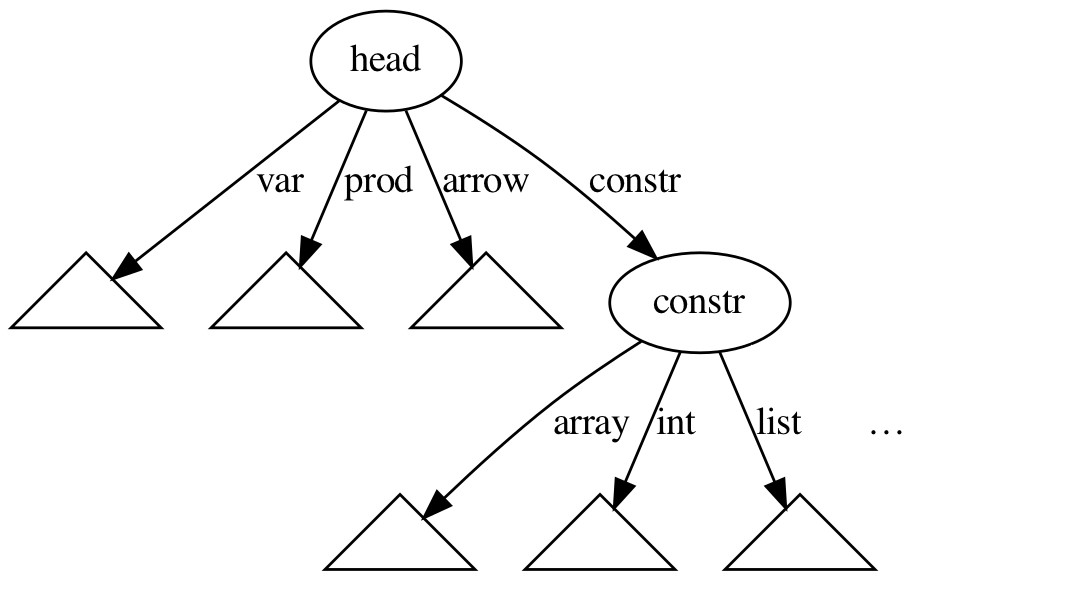
\includegraphics[width=0.6\textwidth]{by_head.png}
  \caption{Feature "by head"}
  \label{fig:byhead}
\end{figure}


% The unification algorithm being already quite optimized, we focused on reducing the number of calls to it. Our approach relies on necessary conditions for unifiability: fast and simple tests before unification. We found discriminating features by observing the statistics of searched libraries. The number and positions of type variables proved particularly instructive.

% Furthermore, we precompute these features into an index. It is built once—it can also be optimized—and can be made incremental. 

%This technique yields very good results for usual queries and can be easily improved by adding new features to the \textit{trie}.

%=================================================================

\section{Conclusion}

We have presented a function retrieval system for OCaml. By combining unification modulo isomorphism and smart indexing techniques, it can efficiently manage a large database. We believe this tool to be useful and practical for programmers. Integration into common editors would ease their move.

%=================================================================

\printbibliography

\end{document}

%%% Local Variables:
%%% mode: latex
%%% TeX-master: t
%%% TeX-command-extra-options: "-shell-escape"
%%% End:
